\section{Dokumentation}
\subsection{Forklar hvad arv er}

\subsection{Forklar hvad abtract betyder}

\subsection{Fortæl hvad det hedder hvis alle fieldklasserne har en landOnField metode der gør noget forskelligt}
Hvis alle fieldklasserne gør brug af den samme landOnField metode er det fordi denne metode er en super metode nedarvet til de forskellige subklasser,
dette gør at alle klasserne kan gøre brug af samme metode. Eksempeltvis, hvis vi har en masse dyr som klasser, kat, hund, kanin etc. så kan de alle nedarve super metoden eat() fra 
superklassen som hedder SurvivalRequirements, eftersom disse er metoder alle dyrene får brug for, så vil det give mening at lave det til en superklasse med supermetoder
, så der holdes lav kobling og høj kohæsion, samt undgås kopiring af kode og høj mulighed for genbrug.
\subsection{Dokumentation for test med screenshots}
    \subsection{JUnit test}
        JUnit test er en autonomisreret testmetode. Her skriver/koder man selv en test, som tester java kode. Oftest opbygger man JUnit test ud fra Java klasser.
        Der er mange måder hvorpå man kan bruge JUnit testen. Man kan både skrive testen inden, man kan skrive den efter, man kan lave den på baggrund af indsigt i koden eller uden nogen form til kendskab af programkoden. Det to sidst nævnte kaldes Black- og Whitebox test.
        Her er et eksempel på et stykke udført JUnit test fra vores spil:
            \begin{figure}[h]\label{fig:JUnitTest} %FIGUR 7???
                \advance\leftskip-3cm
                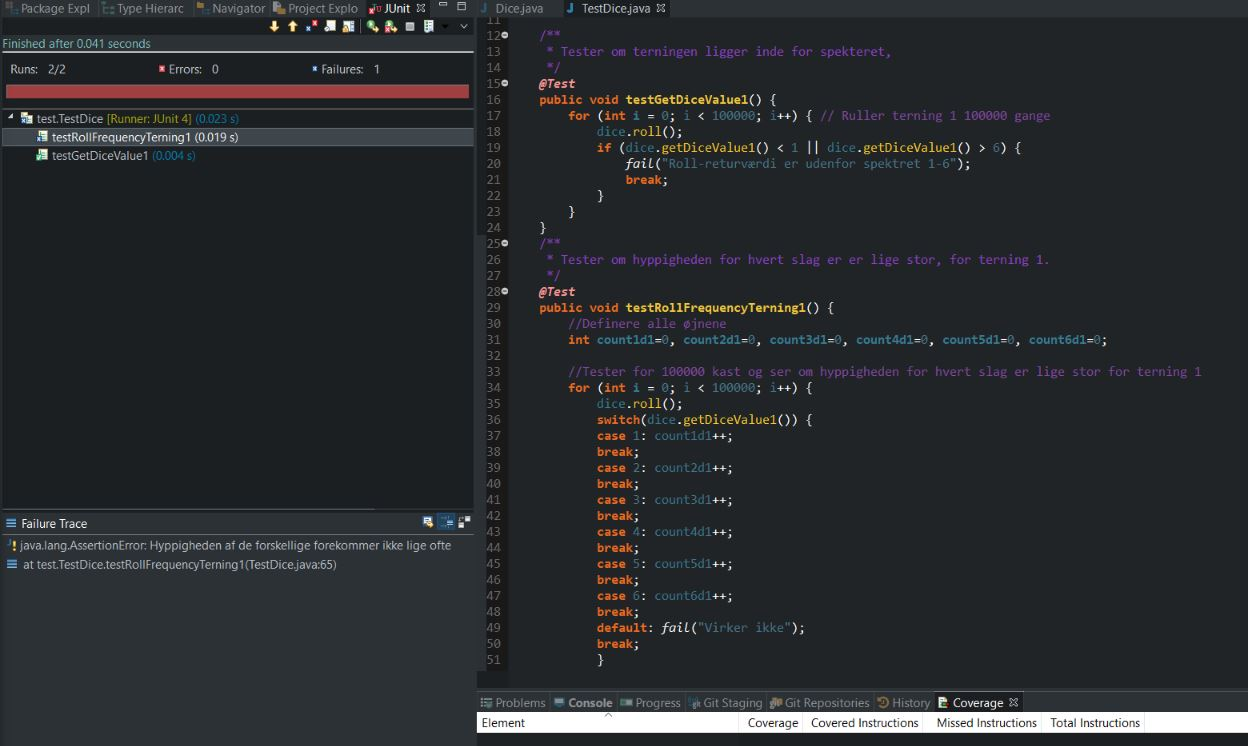
\includegraphics[width=20cm]{fig/JUnitTestDice.jpg}
                \caption{JUnit test udført i Eclipse den 23/11-2017}
            \end{figure}
        Det ser på Figur \ref{fig:JUnitTest} at koden ikke bestod testen, hvor vi også får vist den rette, selv skrevet, fejl besked.

    \subsection{Positiv negativ test}
        Denne test bruges for at teste om systemet kan håndterer 'ugyldige' input, dette kan både være negative som positive værdier, såvel som bogstaver og andre tegn. Denne test forbindes oftest med en eller flere ækvivalensklasse test.
    \subsection{Black- og Whitebox test}
        \textbf{Blackbox test}: Her har du intet kendskab til koden, ud over hvad denne skal kunne gøre. Det er derfor --lige til højre benet-- at teste det faktiske output, mod det forventede output og at teste ækvivalensklasserne.
        \textbf{Whitebox test}: Her opstiller man tests på baggrund af koden og dens opbygning. Man vil med disse tests teste hele koden, altså alle instruktioner, forgreninger og stier, som koden kan blive udført i. Dette er ikke altid muligt med \textit{BlackBox testen} , da man her ikke har et indblik i koden.

\subsection{Dokumentation for overholdt GRASP}
